\begin{frame}[fragile]
\frametitle{Direct State Access}
	\begin{figure}[h]
	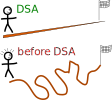
\includegraphics[width=8cm,keepaspectratio]{pics/dsa.pdf}
	\end{figure}
\end{frame}

\begin{frame}
  \frametitle{Direct State Access}
  \begin{itemize}
    \item Since OpenGL 4.5, Khronos added large extension into core profile - Direct State Access.
    \item DSA adds a lot of new functions for direct manipulation of objects.
    \item Bind to modify paradigm will be deprecated in the future.
  \end{itemize}
  Old approach:
  \begin{enumerate}
    \item Backup object id that is currently bound to target.
    \item Bind new object to target.
    \item Execute operation on target.
    \item Rebind backup to target.
  \end{enumerate}
  New approach:
  \begin{enumerate}
    \item Execute operation on object.
  \end{enumerate}
\end{frame}

\begin{frame}
  \frametitle{Direct State Access}
  \begin{itemize}
    \item DSA is easier and follow common sense.
    \item DSA does not break bindings.
    \item DSA is faster, less state switching.
    \item Target is replaced with object id in most OpenGL functions.
    \item DSA exists as extension for a long time - it is supported on all GPUs
  \end{itemize}
\end{frame}

\begin{frame}[fragile]
  \frametitle{Direct State Access - examples}
    Bind to modify:
    {\scriptsize
    \begin{minted}[frame=lines]{c++}
GLint old;
glGenRenderbuffers(1,&RBO);
glGetIntegerv(GL_RENDERBUFFER_BINDING,&old);
glBindRenderbuffer(GL_RENDERBUFFER,RBO);
glRenderbufferStorage(GL_RENDERBUFFER,internalFormat,width,height);
glBindRenderbuffer(GL_RENDERBUFFER,old);
    \end{minted}
    }
    Direct state access:
    {\scriptsize
    \begin{minted}[frame=lines]{c++}
glCreateRenderbuffers(1,&RBO);
glNamedRenderbufferStorage(RBO,internalFormat,width,height);
    \end{minted}
    }
\end{frame}

\begin{frame}[fragile]
  \frametitle{Direct State Access - examples}
    Bind to modify:
    {\scriptsize
    \begin{minted}[frame=lines]{c++}
glBindFramebuffer(GL_READ_FRAMEBUFFER,fbo);
glBindFramebuffer(GL_DRAW_FRAMEBUFFER,0);
glBlitFramebuffer(0,0,width,height,0,0,width,height,
  GL_COLOR_BUFFER_BIT,GL_NEAREST);
    \end{minted}
    }
    Direct state access:
    {\scriptsize
    \begin{minted}[frame=lines]{c++}
glBlitNamedFramebuffer(fbo,0,0,0,width,height,0,0,width,height,
  GL_COLOR_BUFFER_BIT,GL_NEAREST);
    \end{minted}
    }
\end{frame}

\begin{frame}[fragile]
  \frametitle{Direct State Access - confusion}
  \begin{itemize}
    \item Some OpenGL action have 2 or even 3 alternative commands.
    \item A lot of functions is redundant.
    \item Confusion in texture, vao commands
  \end{itemize}
    {\tiny
    \begin{minted}[frame=lines]{c++}
glFramebufferTexture
glFramebufferTexture1D;
glFramebufferTexture2D;
glFramebufferTexture3D;
glFramebufferTextureLayer;
glNamedFramebufferTexture;
glNamedFramebufferTextureLayer;
    \end{minted}
    }
    {\tiny
    \begin{minted}[frame=lines]{c++}
glVertexArrayBindingDivisor
glVertexAttribDivisor
glVertexBindingDivisor
    \end{minted}
    }
    {\tiny
    \begin{minted}[frame=lines]{c++}
glTexImage2D
glTexStorage2D
glTextureStorage2D
    \end{minted}
    }
\end{frame}

